\chapter{Ferromagnetic Nanorods as a Magnetic Nonlinear Beacon}

\label{ch:nanorod}

In order to generate a harmonic response, the nonlinear object must possess inherent nonlinearity in its material properties. Since TR uses electromagnetic waves, we are interested in possble nonlinear electric or magnetic properties. In this section, we discuss a potential magnetic nonlinear object in the form of ferromagnetic nanorods. These nanorods have a nonlinear magnetization curve, as shown in \todo{add figure for hysteresis loop}. This means that the B-field generated from an interrogation signal should have a harmonic response that we may use for NLTR. 

While the usage of diodes as a nonlinear object had been well-documented, the usage of ferromagnets as a nonlinear object had not. Due to this, we had to perform preliminary experiments on the ferromagnetic nanorods in order to verify that the nonlinear response was strong enough to ensure success NLTR experiments. 

This preliminary expertiment consisted of sending a pulse signal into an antenna with the ferromagnetic nanorods attached to them and recording the response signal. By transforming the response signal to the frequency domain, we were able to easily identify whether or not a 2f harmonic was generated. 

\begin{figure}[h!]
    \centering
    \begin{subfigure}{0.45\textwidth}
        \centering
        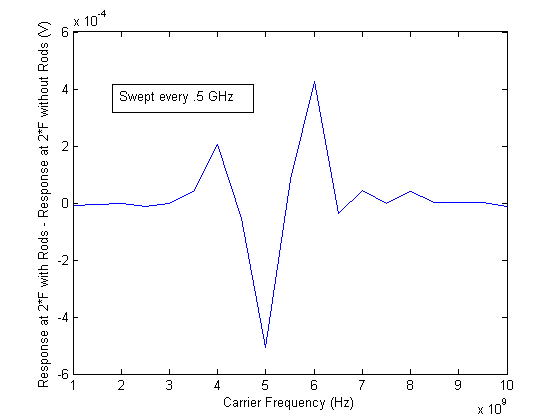
\includegraphics[width=1.0\linewidth]{nanorod/exp-1}
        \caption[]{}
        \label{fig:nanorod-exp-1}
    \end{subfigure}
        \begin{subfigure}{0.45\textwidth}
        \centering
        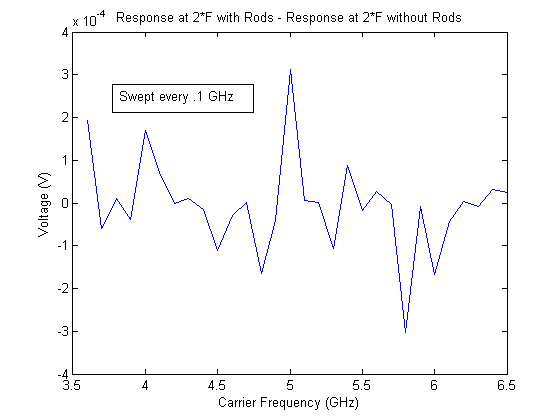
\includegraphics[width=1.0\linewidth]{nanorod/exp-2}
        \caption[]{}
        \label{fig:nanorod-exp-2}
    \end{subfigure}
        \begin{subfigure}{0.45\textwidth}
        \centering
        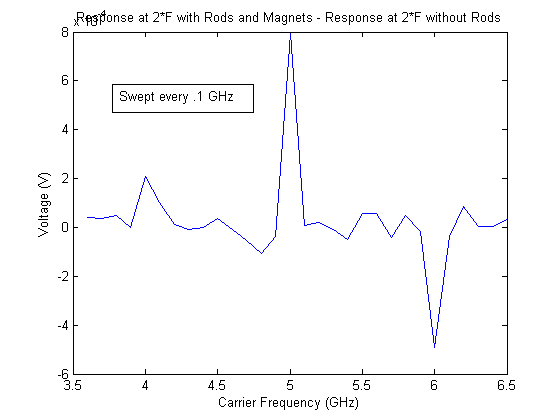
\includegraphics[width=1.0\linewidth]{nanorod/exp-3}
        \caption[]{}
        \label{fig:nanorod-exp-3}
    \end{subfigure}
        \begin{subfigure}{0.45\textwidth}
        \centering
        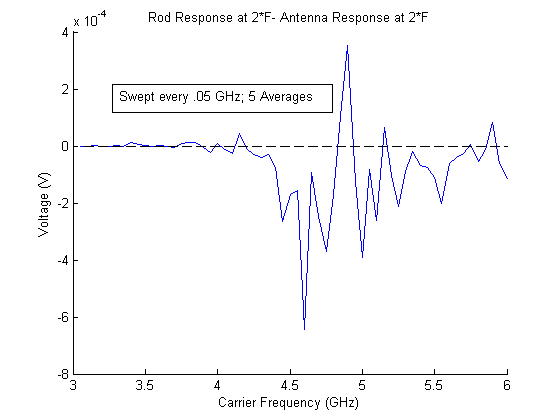
\includegraphics[width=1.0\linewidth]{nanorod/exp-4}
        \caption[]{}
        \label{fig:nanorod-exp-4}
    \end{subfigure}
    \caption[Ferromagnetic nanorod experimental results]{Experimental results}
    \label{fig:nanorod-results}
\end{figure}

Figure~\ref{fig:nanorod-results}(a)-(d) show the 2f response under a variety of conditions. Although there seem to be peaks in (a) - (d), the peaks are somewhat randomly distributed and are small in magnitude. Due to these two aspects of our preliminary testing, we determined that using ferromagnetic nanorods as a potential magnetic nonlinear object was infeasible for performing NLTR. 

\chapter{Ferromagnetic Nanorods as a Electric Nonlinear Beacon}
